% Options for packages loaded elsewhere
\PassOptionsToPackage{unicode}{hyperref}
\PassOptionsToPackage{hyphens}{url}
\PassOptionsToPackage{dvipsnames,svgnames,x11names}{xcolor}
%
\documentclass[
  letterpaper,
]{report}

\usepackage{amsmath,amssymb}
\usepackage{iftex}
\ifPDFTeX
  \usepackage[T1]{fontenc}
  \usepackage[utf8]{inputenc}
  \usepackage{textcomp} % provide euro and other symbols
\else % if luatex or xetex
  \usepackage{unicode-math}
  \defaultfontfeatures{Scale=MatchLowercase}
  \defaultfontfeatures[\rmfamily]{Ligatures=TeX,Scale=1}
\fi
\usepackage{lmodern}
\ifPDFTeX\else  
    % xetex/luatex font selection
\fi
% Use upquote if available, for straight quotes in verbatim environments
\IfFileExists{upquote.sty}{\usepackage{upquote}}{}
\IfFileExists{microtype.sty}{% use microtype if available
  \usepackage[]{microtype}
  \UseMicrotypeSet[protrusion]{basicmath} % disable protrusion for tt fonts
}{}
\makeatletter
\@ifundefined{KOMAClassName}{% if non-KOMA class
  \IfFileExists{parskip.sty}{%
    \usepackage{parskip}
  }{% else
    \setlength{\parindent}{0pt}
    \setlength{\parskip}{6pt plus 2pt minus 1pt}}
}{% if KOMA class
  \KOMAoptions{parskip=half}}
\makeatother
\usepackage{xcolor}
\usepackage[top=30mm,left=20mm,heightrounded]{geometry}
\setlength{\emergencystretch}{3em} % prevent overfull lines
\setcounter{secnumdepth}{-\maxdimen} % remove section numbering
% Make \paragraph and \subparagraph free-standing
\makeatletter
\ifx\paragraph\undefined\else
  \let\oldparagraph\paragraph
  \renewcommand{\paragraph}{
    \@ifstar
      \xxxParagraphStar
      \xxxParagraphNoStar
  }
  \newcommand{\xxxParagraphStar}[1]{\oldparagraph*{#1}\mbox{}}
  \newcommand{\xxxParagraphNoStar}[1]{\oldparagraph{#1}\mbox{}}
\fi
\ifx\subparagraph\undefined\else
  \let\oldsubparagraph\subparagraph
  \renewcommand{\subparagraph}{
    \@ifstar
      \xxxSubParagraphStar
      \xxxSubParagraphNoStar
  }
  \newcommand{\xxxSubParagraphStar}[1]{\oldsubparagraph*{#1}\mbox{}}
  \newcommand{\xxxSubParagraphNoStar}[1]{\oldsubparagraph{#1}\mbox{}}
\fi
\makeatother

\usepackage{color}
\usepackage{fancyvrb}
\newcommand{\VerbBar}{|}
\newcommand{\VERB}{\Verb[commandchars=\\\{\}]}
\DefineVerbatimEnvironment{Highlighting}{Verbatim}{commandchars=\\\{\}}
% Add ',fontsize=\small' for more characters per line
\usepackage{framed}
\definecolor{shadecolor}{RGB}{241,243,245}
\newenvironment{Shaded}{\begin{snugshade}}{\end{snugshade}}
\newcommand{\AlertTok}[1]{\textcolor[rgb]{0.68,0.00,0.00}{#1}}
\newcommand{\AnnotationTok}[1]{\textcolor[rgb]{0.37,0.37,0.37}{#1}}
\newcommand{\AttributeTok}[1]{\textcolor[rgb]{0.40,0.45,0.13}{#1}}
\newcommand{\BaseNTok}[1]{\textcolor[rgb]{0.68,0.00,0.00}{#1}}
\newcommand{\BuiltInTok}[1]{\textcolor[rgb]{0.00,0.23,0.31}{#1}}
\newcommand{\CharTok}[1]{\textcolor[rgb]{0.13,0.47,0.30}{#1}}
\newcommand{\CommentTok}[1]{\textcolor[rgb]{0.37,0.37,0.37}{#1}}
\newcommand{\CommentVarTok}[1]{\textcolor[rgb]{0.37,0.37,0.37}{\textit{#1}}}
\newcommand{\ConstantTok}[1]{\textcolor[rgb]{0.56,0.35,0.01}{#1}}
\newcommand{\ControlFlowTok}[1]{\textcolor[rgb]{0.00,0.23,0.31}{\textbf{#1}}}
\newcommand{\DataTypeTok}[1]{\textcolor[rgb]{0.68,0.00,0.00}{#1}}
\newcommand{\DecValTok}[1]{\textcolor[rgb]{0.68,0.00,0.00}{#1}}
\newcommand{\DocumentationTok}[1]{\textcolor[rgb]{0.37,0.37,0.37}{\textit{#1}}}
\newcommand{\ErrorTok}[1]{\textcolor[rgb]{0.68,0.00,0.00}{#1}}
\newcommand{\ExtensionTok}[1]{\textcolor[rgb]{0.00,0.23,0.31}{#1}}
\newcommand{\FloatTok}[1]{\textcolor[rgb]{0.68,0.00,0.00}{#1}}
\newcommand{\FunctionTok}[1]{\textcolor[rgb]{0.28,0.35,0.67}{#1}}
\newcommand{\ImportTok}[1]{\textcolor[rgb]{0.00,0.46,0.62}{#1}}
\newcommand{\InformationTok}[1]{\textcolor[rgb]{0.37,0.37,0.37}{#1}}
\newcommand{\KeywordTok}[1]{\textcolor[rgb]{0.00,0.23,0.31}{\textbf{#1}}}
\newcommand{\NormalTok}[1]{\textcolor[rgb]{0.00,0.23,0.31}{#1}}
\newcommand{\OperatorTok}[1]{\textcolor[rgb]{0.37,0.37,0.37}{#1}}
\newcommand{\OtherTok}[1]{\textcolor[rgb]{0.00,0.23,0.31}{#1}}
\newcommand{\PreprocessorTok}[1]{\textcolor[rgb]{0.68,0.00,0.00}{#1}}
\newcommand{\RegionMarkerTok}[1]{\textcolor[rgb]{0.00,0.23,0.31}{#1}}
\newcommand{\SpecialCharTok}[1]{\textcolor[rgb]{0.37,0.37,0.37}{#1}}
\newcommand{\SpecialStringTok}[1]{\textcolor[rgb]{0.13,0.47,0.30}{#1}}
\newcommand{\StringTok}[1]{\textcolor[rgb]{0.13,0.47,0.30}{#1}}
\newcommand{\VariableTok}[1]{\textcolor[rgb]{0.07,0.07,0.07}{#1}}
\newcommand{\VerbatimStringTok}[1]{\textcolor[rgb]{0.13,0.47,0.30}{#1}}
\newcommand{\WarningTok}[1]{\textcolor[rgb]{0.37,0.37,0.37}{\textit{#1}}}

\providecommand{\tightlist}{%
  \setlength{\itemsep}{0pt}\setlength{\parskip}{0pt}}\usepackage{longtable,booktabs,array}
\usepackage{calc} % for calculating minipage widths
% Correct order of tables after \paragraph or \subparagraph
\usepackage{etoolbox}
\makeatletter
\patchcmd\longtable{\par}{\if@noskipsec\mbox{}\fi\par}{}{}
\makeatother
% Allow footnotes in longtable head/foot
\IfFileExists{footnotehyper.sty}{\usepackage{footnotehyper}}{\usepackage{footnote}}
\makesavenoteenv{longtable}
\usepackage{graphicx}
\makeatletter
\newsavebox\pandoc@box
\newcommand*\pandocbounded[1]{% scales image to fit in text height/width
  \sbox\pandoc@box{#1}%
  \Gscale@div\@tempa{\textheight}{\dimexpr\ht\pandoc@box+\dp\pandoc@box\relax}%
  \Gscale@div\@tempb{\linewidth}{\wd\pandoc@box}%
  \ifdim\@tempb\p@<\@tempa\p@\let\@tempa\@tempb\fi% select the smaller of both
  \ifdim\@tempa\p@<\p@\scalebox{\@tempa}{\usebox\pandoc@box}%
  \else\usebox{\pandoc@box}%
  \fi%
}
% Set default figure placement to htbp
\def\fps@figure{htbp}
\makeatother

\makeatletter
\@ifpackageloaded{tcolorbox}{}{\usepackage[skins,breakable]{tcolorbox}}
\@ifpackageloaded{fontawesome5}{}{\usepackage{fontawesome5}}
\definecolor{quarto-callout-color}{HTML}{909090}
\definecolor{quarto-callout-note-color}{HTML}{0758E5}
\definecolor{quarto-callout-important-color}{HTML}{CC1914}
\definecolor{quarto-callout-warning-color}{HTML}{EB9113}
\definecolor{quarto-callout-tip-color}{HTML}{00A047}
\definecolor{quarto-callout-caution-color}{HTML}{FC5300}
\definecolor{quarto-callout-color-frame}{HTML}{acacac}
\definecolor{quarto-callout-note-color-frame}{HTML}{4582ec}
\definecolor{quarto-callout-important-color-frame}{HTML}{d9534f}
\definecolor{quarto-callout-warning-color-frame}{HTML}{f0ad4e}
\definecolor{quarto-callout-tip-color-frame}{HTML}{02b875}
\definecolor{quarto-callout-caution-color-frame}{HTML}{fd7e14}
\makeatother
\makeatletter
\@ifpackageloaded{caption}{}{\usepackage{caption}}
\AtBeginDocument{%
\ifdefined\contentsname
  \renewcommand*\contentsname{Table of contents}
\else
  \newcommand\contentsname{Table of contents}
\fi
\ifdefined\listfigurename
  \renewcommand*\listfigurename{List of Figures}
\else
  \newcommand\listfigurename{List of Figures}
\fi
\ifdefined\listtablename
  \renewcommand*\listtablename{List of Tables}
\else
  \newcommand\listtablename{List of Tables}
\fi
\ifdefined\figurename
  \renewcommand*\figurename{Figure}
\else
  \newcommand\figurename{Figure}
\fi
\ifdefined\tablename
  \renewcommand*\tablename{Table}
\else
  \newcommand\tablename{Table}
\fi
}
\@ifpackageloaded{float}{}{\usepackage{float}}
\floatstyle{ruled}
\@ifundefined{c@chapter}{\newfloat{codelisting}{h}{lop}}{\newfloat{codelisting}{h}{lop}[chapter]}
\floatname{codelisting}{Listing}
\newcommand*\listoflistings{\listof{codelisting}{List of Listings}}
\makeatother
\makeatletter
\makeatother
\makeatletter
\@ifpackageloaded{caption}{}{\usepackage{caption}}
\@ifpackageloaded{subcaption}{}{\usepackage{subcaption}}
\makeatother

\usepackage{bookmark}

\IfFileExists{xurl.sty}{\usepackage{xurl}}{} % add URL line breaks if available
\urlstyle{same} % disable monospaced font for URLs
\hypersetup{
  pdftitle={Datathon: Competition},
  pdfauthor={CSUCI Datathon -- Southern California Consortium for Data Science},
  colorlinks=true,
  linkcolor={blue},
  filecolor={Maroon},
  citecolor={Blue},
  urlcolor={Blue},
  pdfcreator={LaTeX via pandoc}}


\title{Datathon: Competition}
\author{CSUCI Datathon -- Southern California Consortium for Data
Science}
\date{2025-04-26}

\begin{document}
\maketitle


\section{Channel Islands}\label{channel-islands}

The \textbf{Channel Islands} are a chain of eight islands located off
the southern coast of California in the Pacific Ocean. They are known
for their stunning natural beauty, ecological richness, and deep
cultural history.

\subsection{The Eight Channel Islands (North to
South)}\label{the-eight-channel-islands-north-to-south}

\begin{enumerate}
\def\labelenumi{\arabic{enumi}.}
\item
  \textbf{San Miguel Island}
\item
  \textbf{Santa Rosa Island}
\item
  \textbf{Santa Cruz Island}
\item
  \textbf{Anacapa Island}
\item
  \textbf{Santa Barbara Island}
\item
  \textbf{San Nicolas Island}
\item
  \textbf{San Clemente Island}
\item
  \textbf{Santa Catalina Island}
\end{enumerate}

\subsection{\texorpdfstring{\href{https://www.nps.gov/chis/index.htm}{Channel
Islands National
Park}}{Channel Islands National Park}}\label{channel-islands-national-park}

\begin{itemize}
\tightlist
\item
  Includes \textbf{five islands}: \emph{San Miguel}, \emph{Santa Rosa},
  \emph{Santa Cruz}, \emph{Anacapa}, and \emph{Santa Barbara}.
\item
  Sometimes called the \textbf{``Galápagos of North America''} for its
  rich biodiversity and many \textbf{endemic species}.
\item
  Accessible only by \textbf{boat or small plane}.
\item
  Ideal for hiking, kayaking, camping, and wildlife observation.
\end{itemize}

\subsection{Cultural and Historical
Significance}\label{cultural-and-historical-significance}

\begin{itemize}
\tightlist
\item
  Originally inhabited by
  \href{https://www.nps.gov/chis/learn/historyculture/nativeinhabitants.htm\#:~:text=With\%20a\%20current\%20population\%20nearly,organized\%20Chumash\%20tribal\%20groups\%20exist}{\textbf{Chumash}
  and \textbf{Tongva}} indigenious groups for thousands of years.
\item
  Home to important archaeological and cultural heritage sites.
\end{itemize}

\section{\texorpdfstring{Island Fox (\emph{Urocyon
littoralis})}{Island Fox (Urocyon littoralis)}}\label{island-fox-urocyon-littoralis}

The \textbf{island fox} is a small, charismatic canid species
\textbf{endemic} to six of the eight \textbf{Channel Islands} off the
coast of southern California. It's one of the best examples of
\textbf{island dwarfism}, having evolved from the mainland gray fox
(\emph{Urocyon cinereoargenteus}) to become significantly smaller.

In the \textbf{1990s}, several island fox populations faced \textbf{near
extinction} due to golden eagle predation, canine distemper virus, and
habitat degradation. The island fox was listed as endangered in 2004.
Recovery efforts of the island fox included removal of golden eagles,
vaccination and captive breeding programs, reintroduction of native bald
eagles, and habitat restoration.

\section{Competition}\label{competition}

For the competition, you will investigate one of the two sections,
\hyperref[fox-weight]{Fox Weight} or \hyperref[fox-rs]{Fox Reproductive
Status}. Follow the guidelines in the section of your choice and
complete one of the challenges. \textbf{You may also analyze the data in
any other way or work on the other section, but it is not necessary.}
Afterwards, create a presentation using google slides. Share the slides
to the lead instructor in the classroom. They will provide their email
on the board.

\subsection{Analysis}\label{analysis}

Using the
\href{https://www.inqs.info/ci_datathon_25/tutorial.html}{tutorial} and
example analysis, complete at least one of the challenges.

\subsection{Slides and Presentation}\label{slides-and-presentation}

The slides will be used for a presentation, in the last 30 minutes. You
should have no more than 5 slides displaying what your findings are.
Here is an example of the slides you should submit:

\begin{enumerate}
\def\labelenumi{\arabic{enumi}.}
\tightlist
\item
  Title Slide

  \begin{itemize}
  \tightlist
  \item
    Come up with a creative title for your analysis.
  \item
    Include the names of all your group members.
  \item
    Include Team Name
  \item
    Provide what you have analyzed
  \end{itemize}
\item
  Numerical Results

  \begin{itemize}
  \tightlist
  \item
    Provide information about the results you found.
  \end{itemize}
\item
  Plots

  \begin{itemize}
  \tightlist
  \item
    Provide any plots.
  \end{itemize}
\item
  Conclusions

  \begin{itemize}
  \tightlist
  \item
    Answer your research question.
  \end{itemize}
\end{enumerate}

Examples can be found \href{}{here} and
\href{https://docs.google.com/presentation/d/1HefRJoGvXEPM7EuhP6JONAQtaxWXlJ629W5KTrP2r68/edit?usp=sharing}{here}.

\section{Data and Prep}\label{data-and-prep}

The data provided is part of an ongoing longitudinal study from 2014 to
2016 of trap monitoring. This resulted in collection of 4,975 recorded
trap observations, which may have contained a fox or not. Other
information collected from the fox were Sex, Age Class, Weight, Body
Condition, Reproductive Status, and Vaccinations. Information of the
data collected can be found in the
\href{https://www.inqs.info/ci_datathon_25/codebook_19052696}{Databook}.

\textbf{You can download the data and script files \href{}{here}.}

\subsection{Loading Packages}\label{loading-packages}

\begin{Shaded}
\begin{Highlighting}[]
\FunctionTok{library}\NormalTok{(tidyverse)}
\end{Highlighting}
\end{Shaded}

\begin{verbatim}
-- Attaching core tidyverse packages ------------------------ tidyverse 2.0.0 --
v dplyr     1.1.4     v readr     2.1.5
v forcats   1.0.0     v stringr   1.5.1
v ggplot2   3.5.1     v tibble    3.2.1
v lubridate 1.9.4     v tidyr     1.3.1
v purrr     1.0.4     
-- Conflicts ------------------------------------------ tidyverse_conflicts() --
x dplyr::filter() masks stats::filter()
x dplyr::lag()    masks stats::lag()
i Use the conflicted package (<http://conflicted.r-lib.org/>) to force all conflicts to become errors
\end{verbatim}

\subsection{Loading Data}\label{loading-data}

We will need to load the data into R using the \texttt{read\_csv}
function.

\begin{Shaded}
\begin{Highlighting}[]
\NormalTok{df }\OtherTok{\textless{}{-}}\NormalTok{ cidf }\OtherTok{\textless{}{-}} \FunctionTok{read\_csv}\NormalTok{(}\StringTok{"data\_for\_csuci\_datathon\_2014\_2016.csv"}\NormalTok{) }\CommentTok{\# Loads the Data Set into the objects df and cidf}
\end{Highlighting}
\end{Shaded}

\begin{verbatim}
Rows: 4975 Columns: 16
-- Column specification --------------------------------------------------------
Delimiter: ","
chr  (9): Island, GridCode, TrapResult, Pittag, CaptureType, Sex, Weight_uni...
dbl  (6): SamplingYear, NightNumber, TrapNumber, AgeClass, Weight, BodyCondi...
dttm (1): TrapDate

i Use `spec()` to retrieve the full column specification for this data.
i Specify the column types or set `show_col_types = FALSE` to quiet this message.
\end{verbatim}

\subsection{Cleaning Data}\label{cleaning-data}

\subsubsection{Renaming Categories}\label{renaming-categories}

Looking at the \href{}{Databook}, the variables \texttt{Vaccinations},
\texttt{ReproductiveStatus} and \texttt{BodyCondition} have interesting
ways they are coded. In \texttt{Vaccinations}, missing values
(\texttt{NA}) are considered as not vaccinated; therefore, changing the
missing to ``NV'' will ensure that they are correctly classified, see
data book. In \texttt{ReproductiveStatus}, the missing values
(\texttt{NA}) indicate unknown reproductive status. In
\texttt{BodyCondition}, the numerical values 1, 2, 3, 4, and 5,
represent a condition. To make the condition easier, we will convert
them to the categories. Run the code below to alter them:

\begin{Shaded}
\begin{Highlighting}[]
\NormalTok{df }\OtherTok{\textless{}{-}}\NormalTok{ df }\SpecialCharTok{|\textgreater{}} \FunctionTok{mutate}\NormalTok{( }\CommentTok{\# Will change the variables in the df data set}
    \AttributeTok{Vaccinations =} \FunctionTok{case\_when}\NormalTok{(}\FunctionTok{is.na}\NormalTok{(Vaccinations) }\SpecialCharTok{\textasciitilde{}} \StringTok{"NV"}\NormalTok{, }\AttributeTok{.default =}\NormalTok{ Vaccinations), }\CommentTok{\# Reclassifies Missing Data in Vaccination as "N" per code book.}
    \AttributeTok{ReproductiveStatus =} \FunctionTok{case\_when}\NormalTok{(}\FunctionTok{is.na}\NormalTok{(ReproductiveStatus) }\SpecialCharTok{\textasciitilde{}} \StringTok{"UN"}\NormalTok{, }\AttributeTok{.default =}\NormalTok{ ReproductiveStatus), }\CommentTok{\# Reclassifies Missing Data in Vaccination as "N" per code book.}
    \AttributeTok{BodyCondition =} \FunctionTok{case\_when}\NormalTok{( }\CommentTok{\# Begins to modify BodyCondition}
        \FunctionTok{as.character}\NormalTok{(BodyCondition) }\SpecialCharTok{==} \StringTok{"1"} \SpecialCharTok{\textasciitilde{}} \StringTok{"emaciated"}\NormalTok{, }\CommentTok{\# Changes 1 to emaciated}
        \FunctionTok{as.character}\NormalTok{(BodyCondition) }\SpecialCharTok{==} \StringTok{"2"} \SpecialCharTok{\textasciitilde{}} \StringTok{"thin"}\NormalTok{, }\CommentTok{\# Changes 2 to thin}
        \FunctionTok{as.character}\NormalTok{(BodyCondition) }\SpecialCharTok{==} \StringTok{"3"} \SpecialCharTok{\textasciitilde{}} \StringTok{"healthy wild"}\NormalTok{, }\CommentTok{\# Changes 3 to healthy wild }
        \FunctionTok{as.character}\NormalTok{(BodyCondition) }\SpecialCharTok{==} \StringTok{"4"} \SpecialCharTok{\textasciitilde{}} \StringTok{"extra fat reserves"}\NormalTok{, }\CommentTok{\# Changes 4 to Extra Fat Reserve}
        \FunctionTok{as.character}\NormalTok{(BodyCondition) }\SpecialCharTok{==} \StringTok{"5"} \SpecialCharTok{\textasciitilde{}} \StringTok{"extreme fat reserves"} \CommentTok{\# Changes 5 to Extreme Fat Reserves}
\NormalTok{        )}
\NormalTok{    )}
\end{Highlighting}
\end{Shaded}

\subsubsection{Missing Values}\label{missing-values}

Several variables in the data set may have missing values. Using the
\texttt{summary()}, we can determine which variables have missing values
by looking at the ``NA's'' category.

\begin{Shaded}
\begin{Highlighting}[]
\FunctionTok{summary}\NormalTok{(df)}
\end{Highlighting}
\end{Shaded}

\begin{verbatim}
    Island           SamplingYear    GridCode        
 Length:4975        Min.   :2014   Length:4975       
 Class :character   1st Qu.:2014   Class :character  
 Mode  :character   Median :2015   Mode  :character  
                    Mean   :2015                     
                    3rd Qu.:2016                     
                    Max.   :2016                     
                                                     
    TrapDate                       NightNumber      TrapNumber    
 Min.   :2014-07-16 00:00:00.00   Min.   :1.000   Min.   :  1.00  
 1st Qu.:2014-08-24 00:00:00.00   1st Qu.:2.000   1st Qu.:  4.00  
 Median :2015-08-12 00:00:00.00   Median :3.000   Median :  8.00  
 Mean   :2015-08-25 01:31:27.92   Mean   :3.392   Mean   : 18.87  
 3rd Qu.:2016-08-18 00:00:00.00   3rd Qu.:5.000   3rd Qu.: 11.00  
 Max.   :2016-11-30 00:00:00.00   Max.   :6.000   Max.   :108.00  
                                                                  
  TrapResult           Pittag          CaptureType            Sex           
 Length:4975        Length:4975        Length:4975        Length:4975       
 Class :character   Class :character   Class :character   Class :character  
 Mode  :character   Mode  :character   Mode  :character   Mode  :character  
                                                                            
                                                                            
                                                                            
                                                                            
    AgeClass         Weight       Weight_units       BodyCondition     
 Min.   :0.000   Min.   :  0.72   Length:4975        Length:4975       
 1st Qu.:1.000   1st Qu.:  1.73   Class :character   Class :character  
 Median :1.000   Median :  2.02   Mode  :character   Mode  :character  
 Mean   :1.557   Mean   : 49.49                                        
 3rd Qu.:3.000   3rd Qu.:  2.30                                        
 Max.   :4.000   Max.   :910.00                                        
 NA's   :2840    NA's   :2808                                          
 ReproductiveStatus Vaccinations      
 Length:4975        Length:4975       
 Class :character   Class :character  
 Mode  :character   Mode  :character  
                                      
                                      
                                      
                                      
\end{verbatim}

We notice that the variables \texttt{AgeClass}, \texttt{Weight}, and
\texttt{BodyCondition} have missing values. \textbf{For this analysis,
we will remove the missing values (\texttt{NA}).}

\begin{Shaded}
\begin{Highlighting}[]
\NormalTok{df }\OtherTok{\textless{}{-}} \FunctionTok{drop\_na}\NormalTok{(df, AgeClass, Weight, BodyCondition) }\CommentTok{\# Removes the missing values (NA) using the variables AgeClass, Weight, and BodyCondition}
\end{Highlighting}
\end{Shaded}

\textbf{After cleaning the data, this should result in 1,967 recorded
foxes!}

\section{Fox Weight Analysis}\label{fox-weight}

Imagine you're a field biologist tracking animal health across the
remote Santa Rosa and San Miguel Islands. You've noticed that some
animals seem heavier in certain years---but is it just your imagination,
or is there a real trend?

The \texttt{Weght} variable contains information of the Fox's weight in
killogrgms. Let's start by calculating the mean weight and standard
deviation of weight using \texttt{mean()} and \texttt{sd()} functions:

\begin{Shaded}
\begin{Highlighting}[]
\NormalTok{mean\_weight}\OtherTok{\textless{}{-}}\FunctionTok{mean}\NormalTok{(df}\SpecialCharTok{$}\NormalTok{Weight)}
\NormalTok{sd\_weight}\OtherTok{\textless{}{-}}\FunctionTok{sd}\NormalTok{(df}\SpecialCharTok{$}\NormalTok{Weight)}
\NormalTok{mean\_weight}
\end{Highlighting}
\end{Shaded}

\begin{verbatim}
[1] 1.940275
\end{verbatim}

\begin{Shaded}
\begin{Highlighting}[]
\NormalTok{sd\_weight }\CommentTok{\#printing the values}
\end{Highlighting}
\end{Shaded}

\begin{verbatim}
[1] 0.4140872
\end{verbatim}

We see that mean weght of fox is about 1.9 kg with standard deviation
about .41 kg.

We will use the \texttt{table()} and \texttt{prop.table()} function to
get the frequencies and proportions for the \texttt{Sex}.

\begin{Shaded}
\begin{Highlighting}[]
\NormalTok{count\_df }\OtherTok{\textless{}{-}} \FunctionTok{table}\NormalTok{(df}\SpecialCharTok{$}\NormalTok{Sex) }\CommentTok{\# Using the \textquotesingle{}Sex\textquotesingle{} variable from the \textasciigrave{}df\textasciigrave{} data set, we count the frequencies of each category with the table function and storing it in rs\_df.}
\NormalTok{count\_df }\CommentTok{\# Printing out the contents of "rs\_df"}
\end{Highlighting}
\end{Shaded}

\begin{verbatim}

Female   Male 
   923   1044 
\end{verbatim}

Using the \texttt{table()} function, we can see that there are 923
female and 1044 male Foxes.

\begin{Shaded}
\begin{Highlighting}[]
\FunctionTok{prop.table}\NormalTok{(count\_df) }\CommentTok{\# Computing the Proportions of "rs\_df"}
\end{Highlighting}
\end{Shaded}

\begin{verbatim}

   Female      Male 
0.4692425 0.5307575 
\end{verbatim}

Using the \texttt{prop.table()} function, we can see that that there are
slightly more male Foxes (about 53\%) vs.~female Foxes (about 47\%).

We can visualize the data using the \texttt{ggplot} functions:

\begin{Shaded}
\begin{Highlighting}[]
\FunctionTok{ggplot}\NormalTok{(df) }\SpecialCharTok{+} \CommentTok{\# Setting up the data to create a plot.}
  \FunctionTok{geom\_bar}\NormalTok{(}\FunctionTok{aes}\NormalTok{(Sex)) }\CommentTok{\# Creating a bar chart based on the variable "ReproductiveStatus"}
\end{Highlighting}
\end{Shaded}

\pandocbounded{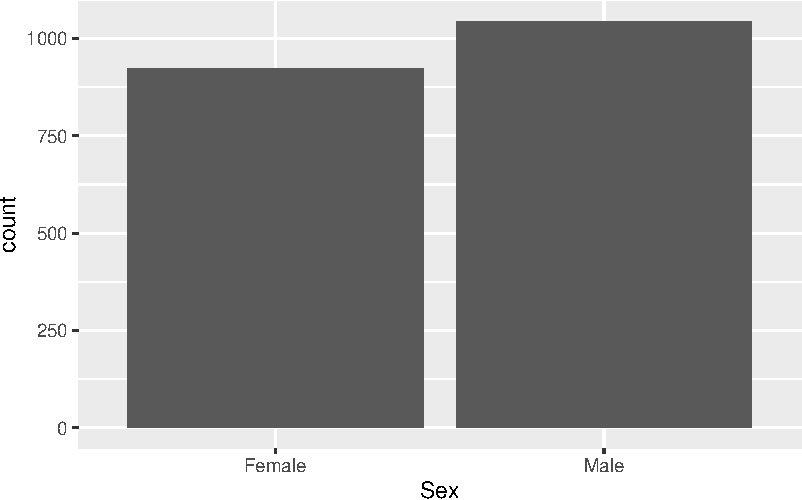
\includegraphics[keepaspectratio]{datathon_files/figure-pdf/unnamed-chunk-9-1.pdf}}

The bar plot demonstrates that there are more males than females.

\subsection{Weight vs Sex}\label{weight-vs-sex}

Let's visualize the variable \texttt{Weight} and \texttt{Sex} with a box
plot using \texttt{ggplot}:

\begin{Shaded}
\begin{Highlighting}[]
\FunctionTok{ggplot}\NormalTok{(df, }\FunctionTok{aes}\NormalTok{(}\AttributeTok{x =}\NormalTok{ Sex, }\AttributeTok{y =}\NormalTok{ Weight)) }\SpecialCharTok{+}
  \FunctionTok{geom\_boxplot}\NormalTok{() }\SpecialCharTok{+}
  \FunctionTok{labs}\NormalTok{(}
    \AttributeTok{title =} \StringTok{"Boxplot of Weight by Sex"}\NormalTok{,}
    \AttributeTok{x =} \StringTok{"Sex"}\NormalTok{,}
    \AttributeTok{y =} \StringTok{"Weight"}
\NormalTok{  )}
\end{Highlighting}
\end{Shaded}

\pandocbounded{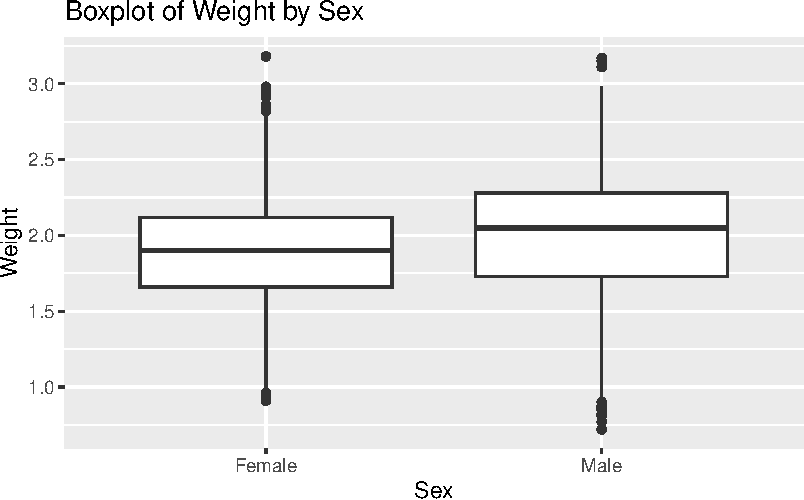
\includegraphics[keepaspectratio]{datathon_files/figure-pdf/unnamed-chunk-10-1.pdf}}

From the box plot we see that male Foxs are slightly heavier than female
Foxes.

We can use \texttt{group\_by()} function to separate male from female
population and calculate mean and standard deviation separately:

\begin{Shaded}
\begin{Highlighting}[]
\NormalTok{weight\_summary }\OtherTok{\textless{}{-}}\NormalTok{ df }\SpecialCharTok{\%\textgreater{}\%}
  \FunctionTok{group\_by}\NormalTok{(Sex) }\SpecialCharTok{\%\textgreater{}\%}
  \FunctionTok{summarise}\NormalTok{(}
    \AttributeTok{mean\_weight =} \FunctionTok{mean}\NormalTok{(Weight),}
    \AttributeTok{sd\_weight =} \FunctionTok{sd}\NormalTok{(Weight),}
    \AttributeTok{.groups =} \StringTok{"drop"}
\NormalTok{  )}
\NormalTok{weight\_summary}
\end{Highlighting}
\end{Shaded}

\begin{verbatim}
# A tibble: 2 x 3
  Sex    mean_weight sd_weight
  <chr>        <dbl>     <dbl>
1 Female        1.88     0.386
2 Male          1.99     0.431
\end{verbatim}

This table confirms that male Foxes are slightly heavier, about 1.99 kg,
than female Foxes, about 1.88 kg, with standard deviations also slightly
higher for male Foxes.

\subsubsection{Weight vs Sex over time}\label{weight-vs-sex-over-time}

To see weight vs sex trend over time we can use \texttt{group\_by()} and
\texttt{ggplot} functions again:

\begin{Shaded}
\begin{Highlighting}[]
\NormalTok{weight\_summary\_yearly }\OtherTok{\textless{}{-}}\NormalTok{ df }\SpecialCharTok{\%\textgreater{}\%}
  \FunctionTok{group\_by}\NormalTok{(Sex, SamplingYear) }\SpecialCharTok{\%\textgreater{}\%}
  \FunctionTok{summarise}\NormalTok{(}
    \AttributeTok{mean\_weight =} \FunctionTok{mean}\NormalTok{(Weight, }\AttributeTok{na.rm =} \ConstantTok{TRUE}\NormalTok{),}
    \AttributeTok{sd\_weight =} \FunctionTok{sd}\NormalTok{(Weight, }\AttributeTok{na.rm =} \ConstantTok{TRUE}\NormalTok{),}
    \AttributeTok{.groups =} \StringTok{"drop"}
\NormalTok{  ) }\CommentTok{\#group the data by Sex and Year and calculate mean and standard deviation of weight}
\NormalTok{weight\_summary\_yearly}
\end{Highlighting}
\end{Shaded}

\begin{verbatim}
# A tibble: 6 x 4
  Sex    SamplingYear mean_weight sd_weight
  <chr>         <dbl>       <dbl>     <dbl>
1 Female         2014        1.95     0.362
2 Female         2015        1.85     0.409
3 Female         2016        1.86     0.373
4 Male           2014        2.08     0.405
5 Male           2015        1.95     0.451
6 Male           2016        1.99     0.419
\end{verbatim}

From the table we see a downward trend in weight for both females and
males. Let's plot it on the graph:

\begin{Shaded}
\begin{Highlighting}[]
\FunctionTok{ggplot}\NormalTok{(weight\_summary\_yearly, }\FunctionTok{aes}\NormalTok{(}\AttributeTok{x =}\NormalTok{ SamplingYear, }\AttributeTok{y =}\NormalTok{ mean\_weight)) }\SpecialCharTok{+}
  \FunctionTok{geom\_line}\NormalTok{() }\SpecialCharTok{+}
  \FunctionTok{geom\_point}\NormalTok{() }\SpecialCharTok{+}
  \FunctionTok{geom\_errorbar}\NormalTok{(}\FunctionTok{aes}\NormalTok{(}\AttributeTok{ymin =}\NormalTok{ mean\_weight }\SpecialCharTok{{-}}\NormalTok{ sd\_weight,}
                    \AttributeTok{ymax =}\NormalTok{ mean\_weight }\SpecialCharTok{+}\NormalTok{ sd\_weight), }\AttributeTok{width =} \FloatTok{0.2}\NormalTok{) }\SpecialCharTok{+}
  \FunctionTok{facet\_wrap}\NormalTok{(}\SpecialCharTok{\textasciitilde{}}\NormalTok{ Sex) }\SpecialCharTok{+}
  \FunctionTok{labs}\NormalTok{(}
    \AttributeTok{title =} \StringTok{"Average Weight by Year and Sex"}\NormalTok{,}
    \AttributeTok{y =} \StringTok{"Mean Weight"}\NormalTok{,}
    \AttributeTok{x =} \StringTok{"Year"}
\NormalTok{  )}
\end{Highlighting}
\end{Shaded}

\pandocbounded{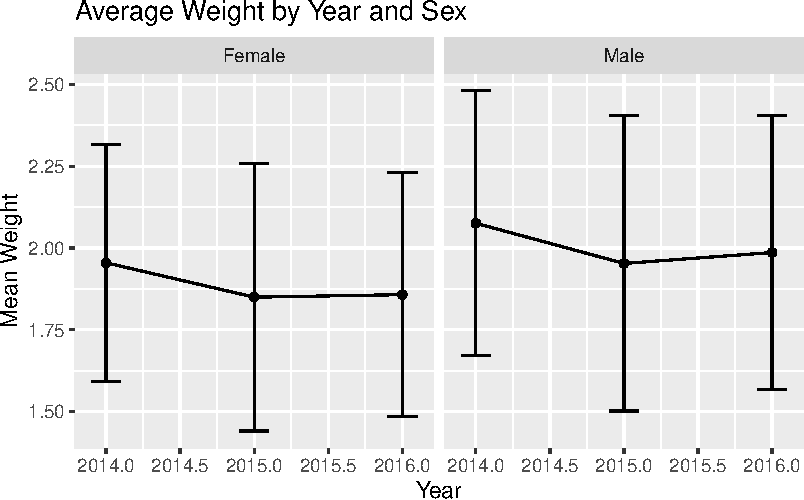
\includegraphics[keepaspectratio]{datathon_files/figure-pdf/unnamed-chunk-13-1.pdf}}

\begin{tcolorbox}[enhanced jigsaw, arc=.35mm, colframe=quarto-callout-note-color-frame, opacityback=0, leftrule=.75mm, coltitle=black, rightrule=.15mm, colbacktitle=quarto-callout-note-color!10!white, left=2mm, titlerule=0mm, bottomrule=.15mm, bottomtitle=1mm, toptitle=1mm, breakable, opacitybacktitle=0.6, toprule=.15mm, title={Weight vs Sex over time by Island}, colback=white]

Take a moment to conduct the same analysis for different
\texttt{Islands} separately and comment on the trends you see:

\begin{Shaded}
\begin{Highlighting}[]
\CommentTok{\#Santa Rosa Fox population }

\NormalTok{SR\_df}\OtherTok{\textless{}{-}}\FunctionTok{filter}\NormalTok{(df,Island}\SpecialCharTok{==}\StringTok{"SRI"}\NormalTok{)}

\CommentTok{\#San Miguel Fox population}
\NormalTok{SM\_df}\OtherTok{\textless{}{-}}\FunctionTok{filter}\NormalTok{(df,Island}\SpecialCharTok{==}\StringTok{"SMI"}\NormalTok{)}
\end{Highlighting}
\end{Shaded}

\end{tcolorbox}

\subsection{Challenges}\label{challenges}

\begin{tcolorbox}[enhanced jigsaw, arc=.35mm, colframe=quarto-callout-tip-color-frame, opacityback=0, leftrule=.75mm, coltitle=black, rightrule=.15mm, colbacktitle=quarto-callout-tip-color!10!white, left=2mm, titlerule=0mm, bottomrule=.15mm, bottomtitle=1mm, toptitle=1mm, breakable, opacitybacktitle=0.6, toprule=.15mm, title={Vaccinations}, colback=white]

Analyse the interaction between \texttt{Weight} and
\texttt{Vaccinations}

\end{tcolorbox}

\begin{tcolorbox}[enhanced jigsaw, arc=.35mm, colframe=quarto-callout-warning-color-frame, opacityback=0, leftrule=.75mm, coltitle=black, rightrule=.15mm, colbacktitle=quarto-callout-warning-color!10!white, left=2mm, titlerule=0mm, bottomrule=.15mm, bottomtitle=1mm, toptitle=1mm, breakable, opacitybacktitle=0.6, toprule=.15mm, title={Body Condition}, colback=white]

Analyse the interaction between \texttt{Weight} and
\texttt{BodyCondition}

\end{tcolorbox}

\section{Fox Reproductive Status Analysis}\label{fox-rs}

The \texttt{ReproductiveStatus} variable contains information of the
Fox's reproductive status when captures. This data is recorded as ``N''
(Not actively reproductive), ``L'' (Lactating), ``SL'' (Signs of
Lactating), and ``TD'' (Testes Distended).

\subsection{Descriptive Statistics}\label{descriptive-statistics}

\subsubsection{Reproductive Status}\label{reproductive-status}

We will use the \texttt{table()} and \texttt{prop.table()} function to
get the frequencies and proportions for the \texttt{ReproductiveStatus}.

\begin{Shaded}
\begin{Highlighting}[]
\NormalTok{rs\_df }\OtherTok{\textless{}{-}} \FunctionTok{table}\NormalTok{(df}\SpecialCharTok{$}\NormalTok{ReproductiveStatus) }\CommentTok{\# Using the \textquotesingle{}ReproductiveStatus\textquotesingle{} variable from the \textasciigrave{}df\textasciigrave{} data set, we count the frequencies of each category with the table function and storing it in rs\_df.}
\NormalTok{rs\_df }\CommentTok{\# Printing out the contents of "rs\_df"}
\end{Highlighting}
\end{Shaded}

\begin{verbatim}

   L   SL   TD   UN 
  18  244 1030  675 
\end{verbatim}

Using the \texttt{table()} function, we can see that there are 3 common
reproductive statuses by Fox: ``L'' at 18, ``SL'' at 244, ``TD'' at
1030, and ``UN'' at 675.

\begin{Shaded}
\begin{Highlighting}[]
\FunctionTok{prop.table}\NormalTok{(rs\_df) }\CommentTok{\# Computing the Proportions of "rs\_df"}
\end{Highlighting}
\end{Shaded}

\begin{verbatim}

          L          SL          TD          UN 
0.009150991 0.124046772 0.523640061 0.343162176 
\end{verbatim}

Using the \texttt{prop.table()} function, we can see that that the most
common status is ``TD'' at 52.4\% and the least common is ``L'' at the
0.9\%. Both ``SL'' and ``UN'' represent 12.4\% and 34.3\% of the data,
respectively.

We can visualize the data using the \texttt{ggplot} functions:

\begin{Shaded}
\begin{Highlighting}[]
\FunctionTok{ggplot}\NormalTok{(df) }\SpecialCharTok{+} \CommentTok{\# Setting up the data to create a plot.}
  \FunctionTok{geom\_bar}\NormalTok{(}\FunctionTok{aes}\NormalTok{(ReproductiveStatus)) }\CommentTok{\# Creating a bar chart based on the variable "ReproductiveStatus"}
\end{Highlighting}
\end{Shaded}

\pandocbounded{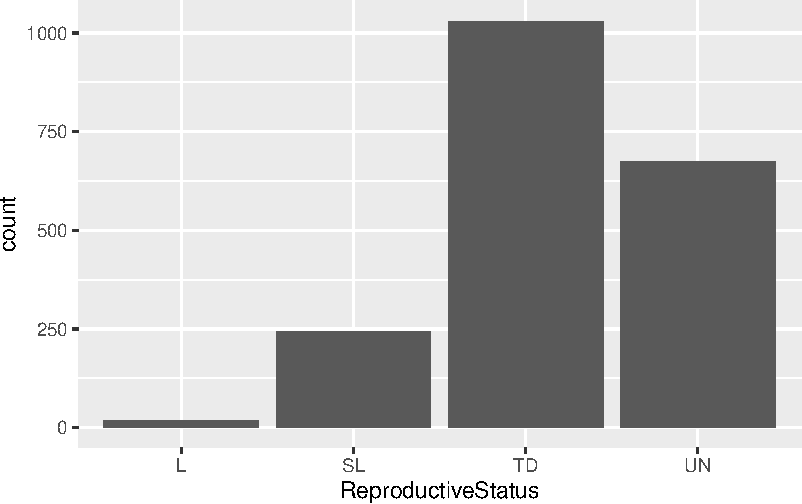
\includegraphics[keepaspectratio]{datathon_files/figure-pdf/unnamed-chunk-17-1.pdf}}

The bar plot demonstrates that ``TD'' is the most common status in the
data, and ``L'' is the least common status in the data.

\begin{tcolorbox}[enhanced jigsaw, arc=.35mm, colframe=quarto-callout-note-color-frame, opacityback=0, leftrule=.75mm, coltitle=black, rightrule=.15mm, colbacktitle=quarto-callout-note-color!10!white, left=2mm, titlerule=0mm, bottomrule=.15mm, bottomtitle=1mm, toptitle=1mm, breakable, opacitybacktitle=0.6, toprule=.15mm, title={Analysing Sex}, colback=white]

Take a moment to conduct the same analysis with the \texttt{Sex}
variable.

\end{tcolorbox}

\subsection{Sex and Reproductive
Status}\label{sex-and-reproductive-status}

Let's compare the frequencies between the variables \texttt{Sex} and
\texttt{Reproductive\ Status}. We will be using the same
\texttt{table()} function:

\begin{Shaded}
\begin{Highlighting}[]
\NormalTok{xy\_df }\OtherTok{\textless{}{-}} \FunctionTok{table}\NormalTok{(df}\SpecialCharTok{$}\NormalTok{ReproductiveStatus, df}\SpecialCharTok{$}\NormalTok{Sex)}
\CommentTok{\# Use the variables "ReproductiveStatus" and "Sex" from the "df" data set}
\CommentTok{\# Use the table function to compute the crosstabs}
\CommentTok{\# Store the results in the xy\_df object}

\NormalTok{xy\_df }\CommentTok{\# Print results out}
\end{Highlighting}
\end{Shaded}

\begin{verbatim}
    
     Female Male
  L      18    0
  SL    244    0
  TD      0 1030
  UN    661   14
\end{verbatim}

The results show that certain categorical combinations between
\texttt{ReproductiveStatus} and \texttt{Sex} are 0, which is to be
expected. The category ``UN'' is found in both Male and Female foxes.
Looking at Female foxes, The most common type is ``UN'', followed by
``SL''. For Male foxes, the most common type was ``TD''.

Let's find the proportions for each the combination of the variables
using the \texttt{prop.table()} function.

\begin{Shaded}
\begin{Highlighting}[]
\FunctionTok{prop.table}\NormalTok{(xy\_df)}
\end{Highlighting}
\end{Shaded}

\begin{verbatim}
    
          Female        Male
  L  0.009150991 0.000000000
  SL 0.124046772 0.000000000
  TD 0.000000000 0.523640061
  UN 0.336044738 0.007117438
\end{verbatim}

We can see that 52.4\% of the data are Male and ``TD'' foxes, 33.6\% of
the data are Female and ``UN'' foxes, and 12.4\% of the data are Female
and ``SL'' foxes.

Let's visualize the variable \texttt{ReproductiveStatus} and
\texttt{Sex} with a stacked bar plot:

\begin{Shaded}
\begin{Highlighting}[]
\FunctionTok{ggplot}\NormalTok{(df) }\SpecialCharTok{+}
  \FunctionTok{geom\_bar}\NormalTok{(}\FunctionTok{aes}\NormalTok{(Sex, }\AttributeTok{fill =}\NormalTok{ ReproductiveStatus))}
\end{Highlighting}
\end{Shaded}

\pandocbounded{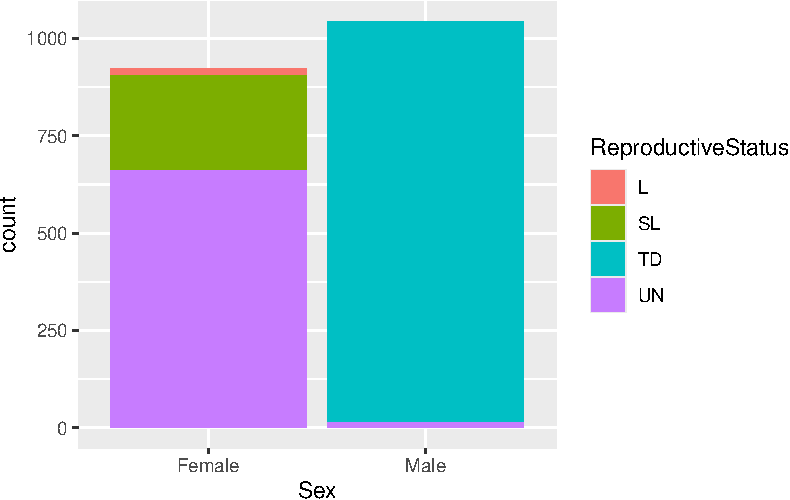
\includegraphics[keepaspectratio]{datathon_files/figure-pdf/unnamed-chunk-20-1.pdf}}

The plot indicate which categories are most dominant in each sex. We can
see that the most dominant reproductive status in Male foxes is testes
distended. For Female foxes, we can see tha tthe most common
reproductive status being unknown.

\subsection{Challenges}\label{challenges-1}

\begin{tcolorbox}[enhanced jigsaw, arc=.35mm, colframe=quarto-callout-note-color-frame, opacityback=0, leftrule=.75mm, coltitle=black, rightrule=.15mm, colbacktitle=quarto-callout-note-color!10!white, left=2mm, titlerule=0mm, bottomrule=.15mm, bottomtitle=1mm, toptitle=1mm, breakable, opacitybacktitle=0.6, toprule=.15mm, title={Age Class}, colback=white]

Analyse the interaction between \texttt{ReproductiveStatus} and
\texttt{AgeClass}

\end{tcolorbox}

\begin{tcolorbox}[enhanced jigsaw, arc=.35mm, colframe=quarto-callout-tip-color-frame, opacityback=0, leftrule=.75mm, coltitle=black, rightrule=.15mm, colbacktitle=quarto-callout-tip-color!10!white, left=2mm, titlerule=0mm, bottomrule=.15mm, bottomtitle=1mm, toptitle=1mm, breakable, opacitybacktitle=0.6, toprule=.15mm, title={Vaccinations}, colback=white]

Analyse the interaction between \texttt{ReproductiveStatus} and
\texttt{Vaccinations}

\end{tcolorbox}

\begin{tcolorbox}[enhanced jigsaw, arc=.35mm, colframe=quarto-callout-warning-color-frame, opacityback=0, leftrule=.75mm, coltitle=black, rightrule=.15mm, colbacktitle=quarto-callout-warning-color!10!white, left=2mm, titlerule=0mm, bottomrule=.15mm, bottomtitle=1mm, toptitle=1mm, breakable, opacitybacktitle=0.6, toprule=.15mm, title={Capture Type}, colback=white]

Analyse the interaction between \texttt{ReproductiveStatus} and
\texttt{Capture\ Type}

\end{tcolorbox}




\end{document}
